
% Template for Elsevier CRC journal article
% version 1.2 dated 09 May 2011

% This file (c) 2009-2011 Elsevier Ltd.  Modifications may be freely made,
% provided the edited file is saved under a different name

% This file contains modifications for Procedia Engineering

% Changes since version 1.1
% - added "procedia" option compliant with ecrc.sty version 1.2a
%   (makes the layout approximately the same as the Word CRC template)
% - added example for generating copyright line in abstract

%-----------------------------------------------------------------------------------

%% This template uses the elsarticle.cls document class and the extension package ecrc.sty
%% For full documentation on usage of elsarticle.cls, consult the documentation "elsdoc.pdf"
%% Further resources available at http://www.elsevier.com/latex

%-----------------------------------------------------------------------------------

%%%%%%%%%%%%%%%%%%%%%%%%%%%%%%%%%%%%%%%%%%%%%%%%%%%%%%%%%%%%%%
%%%%%%%%%%%%%%%%%%%%%%%%%%%%%%%%%%%%%%%%%%%%%%%%%%%%%%%%%%%%%%
%%                                                          %%
%% Important note on usage                                  %%
%% -----------------------                                  %%
%% This file should normally be compiled with PDFLaTeX      %%
%% Using standard LaTeX should work but may produce clashes %%
%%                                                          %%
%%%%%%%%%%%%%%%%%%%%%%%%%%%%%%%%%%%%%%%%%%%%%%%%%%%%%%%%%%%%%%
%%%%%%%%%%%%%%%%%%%%%%%%%%%%%%%%%%%%%%%%%%%%%%%%%%%%%%%%%%%%%%

%% The '3p' and 'times' class options of elsarticle are used for Elsevier CRC
%% The 'procedia' option causes ecrc to approximate to the Word template
\documentclass[3p,times,procedia,number]{elsarticle}
\flushbottom

%% The `ecrc' package must be called to make the CRC functionality available
\usepackage{ecrc}
%\usepackage{amsmath}
\usepackage{amsmath}
\usepackage{amssymb}
\usepackage{bm}
%\usepackage[fleqn]{amsmath}
\usepackage{caption}
\usepackage{ulem}
\usepackage[colorlinks,linkcolor=blue,citecolor=blue,urlcolor=blue]{hyperref}
\usepackage{graphicx} 
\setcounter{totalnumber}{4}
\renewcommand{\textfraction}{0.15}
\renewcommand{\topfraction}{0.85}
\renewcommand{\bottomfraction}{0.65}
\renewcommand{\floatpagefraction}{0.60}
\newcommand{\figref}[1]{\figurename~\ref{#1}}
\usepackage{titlesec}
\titleformat{\chapter}[display]
{\normalfont\Large\bfseries}{\thechapter}{11pt}{\Large}
\titleformat{\section}
{\normalfont\large\bfseries}{\thesection}{11pt}{\large}
\titlespacing*{\chapter}{0pt}{0pt}{15pt} %left, beforesep, aftersep, right
\titlespacing*{\section}{0pt}{3.5ex plus 1ex minus .2ex}{2.3ex plus .2ex}
\usepackage[titletoc]{appendix}
\usepackage{listings}
\makeatletter
\newcommand{\rmnum}[1]{\romannumeral #1}
\newcommand{\Rmnum}[1]{\expandafter\@slowromancap\romannumeral #1@}
\makeatother
\newcommand{\HRule}{\rule{\linewidth}{0.5mm}}
\usepackage{xltxtra}
\usepackage[francais]{babel}
\usepackage[table,xcdraw]{xcolor}
%% The ecrc package defines commands needed for running heads and logos.
%% For running heads, you can set the journal name, the volume, the starting page and the authors

%% set the volume if you know. Otherwise `00'
\volume{00}

%% set the starting page if not 1
\firstpage{1}

%% Give the name of the journal
\journalname{Procedia Engineering}

%% Give the author list to appear in the running head
%% Example \runauth{C.V. Radhakrishnan et al.}
\runauth{Ma Zepeng et al.}

%% The choice of journal logo is determined by the \jid and \jnltitlelogo commands.
%% A user-supplied logo with the name <\jid>logo.pdf will be inserted if present.
%% e.g. if \jid{yspmi} the system will look for a file yspmilogo.pdf
%% Otherwise the content of \jnltitlelogo will be set between horizontal lines as a default logo

%% Give the abbreviation of the Journal.
\jid{proeng}

%% Give a short journal name for the dummy logo (if needed)
%\jnltitlelogo{Procedia Engineering}

%% Hereafter the template follows `elsarticle'.
%% For more details see the existing template files elsarticle-template-harv.tex and elsarticle-template-num.tex.

%% Elsevier CRC generally uses a numbered reference style
%% For this, the conventions of elsarticle-template-num.tex should be followed (included below)
%% If using BibTeX, use the style file elsarticle-num.bst

%% End of ecrc-specific commands
%%%%%%%%%%%%%%%%%%%%%%%%%%%%%%%%%%%%%%%%%%%%%%%%%%%%%%%%%%%%%%%%%%%%%%%%%%

%% The amssymb package provides various useful mathematical symbols

\usepackage{amssymb}
%% The amsthm package provides extended theorem environments
%% \usepackage{amsthm}

%% The lineno packages adds line numbers. Start line numbering with
%% \begin{linenumbers}, end it with \end{linenumbers}. Or switch it on
%% for the whole article with \linenumbers after \end{frontmatter}.
%% \usepackage{lineno}

%% natbib.sty is loaded by default. However, natbib options can be
%% provided with \biboptions{...} command. Following options are
%% valid:

%%   round  -  round parentheses are used (default)
%%   square -  square brackets are used   [option]
%%   curly  -  curly braces are used      {option}
%%   angle  -  angle brackets are used    <option>
%%   semicolon  -  multiple citations separated by semi-colon
%%   colon  - same as semicolon, an earlier confusion
%%   comma  -  separated by comma
%%   numbers-  selects numerical citations
%%   super  -  numerical citations as superscripts
%%   sort   -  sorts multiple citations according to order in ref. list
%%   sort&compress   -  like sort, but also compresses numerical citations
%%   compress - compresses without sorting
%%
%\biboptions{authoryear}

 \biboptions{sort&compress}

% if you have landscape tables
\usepackage[figuresright]{rotating}
%\usepackage{harvard}
% put your own definitions here:x
%   \newcommand{\cZ}{\cal{Z}}
%   \newtheorem{def}{Definition}[section]
%   ...

% add words to TeX's hyphenation exception list
%\hyphenation{author another created financial paper re-commend-ed Post-Script}

% declarations for front matter

\begin{document}

\begin{frontmatter}

%% Title, authors and addresses

%% use the tnoteref command within \title for footnotes;
%% use the tnotetext command for the associated footnote;
%% use the fnref command within \author or \address for footnotes;
%% use the fntext command for the associated footnote;
%% use the corref command within \author for corresponding author footnotes;
%% use the cortext command for the associated footnote;
%% use the ead command for the email address,
%% and the form \ead[url] for the home page:
%%
%% \title{Title\tnoteref{label1}}
%% \tnotetext[label1]{}
%% \author{Name\corref{cor1}\fnref{label2}}
%% \ead{email address}
%% \ead[url]{home page}
%% \fntext[label2]{}
%% \cortext[cor1]{}
%% \address{Address\fnref{label3}}
%% \fntext[label3]{}

\dochead{6th Fatigue Design conference, Fatigue Design 2015}
%% Use \dochead if there is an article header, e.g. \dochead{Short communication}
%% \dochead can also be used to include a conference title, if directed by the editors
%% e.g. \dochead{17th International Conference on Dynamical Processes in Excited States of Solids}

\title{Plastisity and energy dissipation in HCF}

%% use optional labels to link authors explicitly to addresses:
%% \author[label1,label2]{<author name>}
%% \address[label1]{<address>}
%% \address[label2]{<address>}



\author[a]{Ma Zepeng\corref{cor1}}
\author[b]{Patrick Le Tallec}
\author[c]{Habibou Maitournam}

\address[a]{Laboratory of Solid Mechanics, Ecole Polytechnique, 91128 Palaiseau Cedex, France}
\address[b]{Laboratory of Solid Mechanics, Ecole Polytechnique, 91128 Palaiseau Cedex, France}
\address[c]{Department of Mechanical Engineering, ENSTA ParisTech, 91128 Palaiseau Cedex, France}

\begin{abstract}
%% Text of abstract
We study first  different kinematic hardening models. Varies energy based high cycle fatigue criteria have been proposed, but we have to think of a simpler and universal criterion. Our fundamental thought would be assuming the total energy dissipated is constant at failure, regardless of the number of cycles.
 
\end{abstract}

\begin{keyword}
Fatigue; Multi-axial; High cycle; Finite element, Life prediction

%% keywords here, in the form: keyword \sep keyword

%% PACS codes here, in the form: \PACS code \sep code

%% MSC codes here, in the form: \MSC code \sep code
%% or \MSC[2008] code \sep code (2000 is the default)

\end{keyword}
\cortext[cor1]{Corresponding author. Tel.: +33-671-89-3267\\Email address: zepeng.ma@polytechnique.edu }

\end{frontmatter}


\clearpage
\begin{flushleft}
	\textbf{Nomenclature}
	\vspace{6pt}
	\begin{table}[h]
		\begin{tabular}{lllll}
			$D$ & damage variable  &  &  &  \\
			$\sigma_{max}$ & maximum stress &  &  &  \\
			$\overline{\sigma}$ & mean stress &  &  &  \\
			$M(),\alpha()$& functions in the nonlinear continuous damage model &  &  &  \\
			$M_0,a,b,\beta$ & coefficients of the nonlinear continuous damage model &  &  &  \\
			$\sigma_{-1}$ & fatigue limit for fully reversed condition  &  &  &  \\
			$\sigma_{\sigma_m}$ & fatigue limit for a non-zero mean stress  &  &  &  \\
			$\sigma_{a}$ & stress amplitude &  &  &  \\
			$\sigma_{b}$ & back stress  &  &  &  \\
			$\sigma_{u}$ & ultimate tensile stress &  &  &  \\
			$\sigma_{0}$ & a constant yield stress &  &  &  \\
			$\sigma_{Ten,-1}$ & fully reversed endurance limit in tension &  &  &  \\
			$\sigma_{RotBend,-1}$ & fully reversed endurance limit in rotating bending &  &  &  \\
			$\sigma^*$ & stress below which does not initiate observable damage at the microscopic scale &  &  &  \\
			$\langle$ $\rangle$& MacCauley bracket symbol.$\langle$ $\rangle$ is defined as $\langle m\rangle=0$ if $m\leqslant0$ , $\langle m\rangle=m$ if $m>0$&  &  &  \\
			$W_a$ & the volumic density of the elastic strain energy &  &  &  \\
			$N$& current number of cycles &  &  &  \\
			$N_F$& number of cycles to failure &  &  &  \\
			 $ \dot{\varepsilon}_p$ & rate of effective plastic strain &  &  &  \\
			 $\dot{p}$ & accumulated plastic strain rate given as $\sqrt{\frac{2}{3}}||\dot{\varepsilon}_p||$ &  &  &  \\
			 
		\end{tabular}
	\end{table}
\end{flushleft}

\clearpage
\section{Kinematic Hardening Models}
\subsection{Linear Kinematic Hardening}

\begin{figure}[h!]
	\centering
	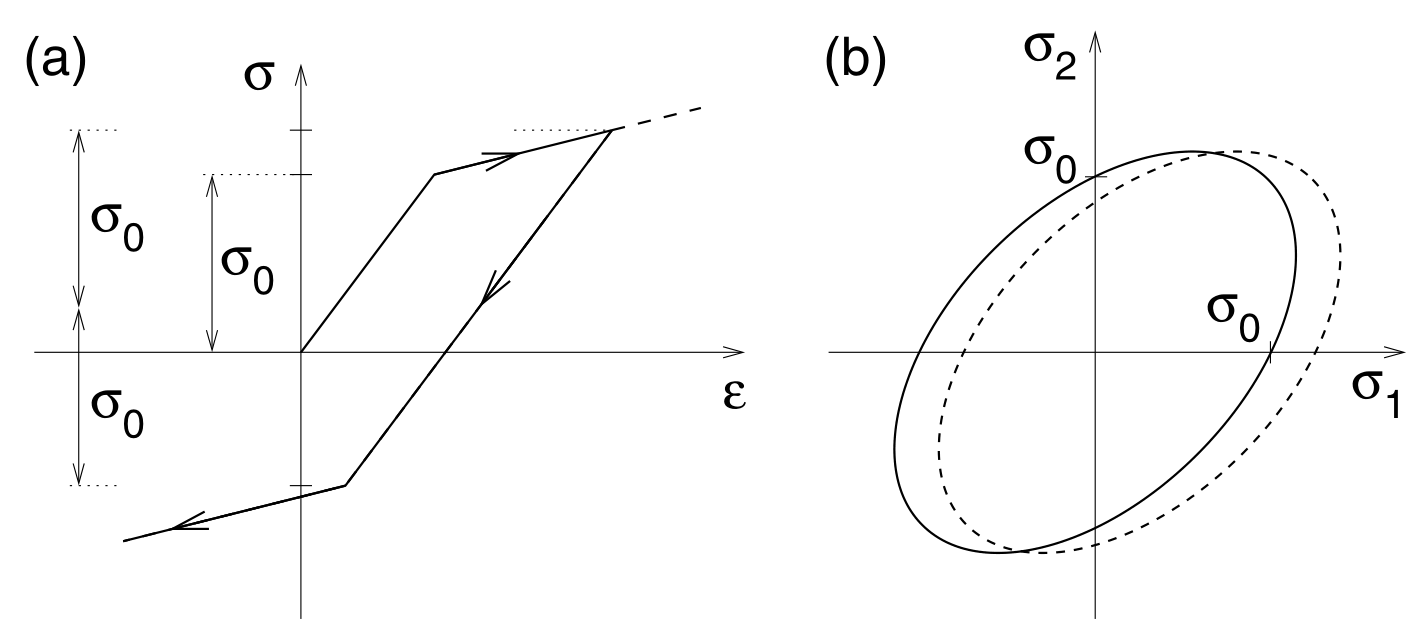
\includegraphics[width=0.8\textwidth]{figures//kinhard.png} 
	\caption{Kinematic hardening: a) uniaxial stress-strain diagram, b) evolution of the
		yield surface in the biaxial stress plane}
	\label{kinhard}
\end{figure}

Kinematic hardening rules are necessary,especially for the case of unloading and cyclic loading.In Kinematic Hardening the current loading surface is assumed not to expand but to move as a rigid body
within the stress space (\figref{kinhard}(b)). The use
of kinematic hardening is, for example, necessary to model the so-called Bauschinger
effect (Bauschinger, 1881). This effect is often observed in metals subjected to cyclic
loading. Even if the magnitudes of the yield stress in tension and in compression
are initially the same, this is no longer the case when the material is preloaded into
the plastic range and then unloaded. For example, after previous yielding in tension,
yielding in compression may start at a stress level lower than the initial yield stress
(\figref{kinhard}(a)).

Kinematic hardening leads to a translation of the loading surface, i.e. to a shift of
the origin of the initial yield surface. If the initial yield surface is described by a yield
function of the form
$$f(\sigma) = F(\sigma) -\sigma_0 $$
the shifted surface is obviously described by
$$f(\sigma,\sigma_b ) = F(\sigma-\sigma_b ) -\sigma_0$$
where $\sigma_b$ is the so-called backstress that represents the center of the shifted elastic
domain and plays the role of a tensorial hardening variable. Now we need a kinematic
hardening law that governs the evolution of the back stress. Melan (1938b) proposed
a law of the form
\begin{equation}
\sigma_b =\overline{H}_K \dot{\varepsilon}_p
\label{lineark}
\end{equation}
where $ \dot{\varepsilon}_p$ is the rate of effective plastic strain. According to which the rate of the back stress is proportional to the plastic strain rate.
The proportionality factor $\overline{H}_K$ is directly related to the plastic modulus and is derived from a simple
monotonic uniaxial curve.The linear hardening law Eq.\eqref{lineark} is often credited to Prager (1955, 1956); we will call it the Melan–Prager hardening rule. 

\subsection{Non-linear Kinematic Hardening}
%\begin{figure}[h!]
%		\includegraphics[width=\textwidth]{figures//kinehardening.gif} 
%		\caption{Dissipated energy in one cycle and number of cycles %to failure when $\beta=-1$}
%		\label{kinehardening}
%\end{figure}
To describe cyclic plasticity, one of the famous model is the non-linear kinematic hardening model formulated by Armstrong and Frederick. It is based on a physical mechanism of strain hardening and dynamic recovery and is capable of simulating the
multiaxial Bauschinger effect (movement of the yield surface in the stress space). Therefore, the model has been examined and implemented in commercial software and finite element analysis.

The Armstrong-Frederick model (AF) is a modification of the Melan–Prager linear kinematic hardening model. The only modification of this simple model is the "recal" term which changes the evolution law for the symmetric backstress tensor $\sigma_b$ from a classical linear kinematic hardening law (Melan–Prager) to a nonlinear kinematic hardening law. The term is proportional to the current back stress multiplied by the norm of the plastic strain rate. According to the Armstrong-Frederick rule, the evolution of the
back stress is governed by the differential equation:

\begin{equation}
\dot{\bm{\sigma}}_b=\underbrace{\overline{H}_K \dot{\varepsilon}_p}_{lin. kin. hardening} -\underbrace{\gamma\dot{p}\bm{\sigma}_b}_{recall - term, nonlinear hardening}
\label{nonlineark}
\end{equation}
where
$\dot{p}$ is the accumulated plastic strain rate given as $\sqrt{\frac{2}{3}}||\dot{\varepsilon}_p||$ . The constants
$\overline{H}_K$
and
$\gamma$
are determined from uniaxial tests.
At the onset of yielding, the
back stress is still zero and Eq.\eqref{nonlineark} gives the same response as the linear hardening
law Eq.\eqref{lineark}. As the back stress develops, the additional term becomes activated and
slows down the rate at which the back stress grows (i.e. reduces the tangent plastic
modulus).

\section{Existing Energy Based Fatigue Models}
\subsection{Energy dissipation based on law of thermodynamics}
In case of shell model. We assume the temperature in the thickness direction does not change. Based on the first and second law of thermodynamics, for any point M, we define $T(M,t)$ is the temperature field of $M$ at time $t$. Its 2D heat transfer function is \cite{yuan2013prediction}:
$$\rho C \frac{\partial T(M,t)}{\partial t}-k\Delta_2 T(M,t)+\frac{2\sigma_e\varepsilon_mT(M,t)^4}{e}+\frac{2h}{e}[T(M,t)-T(M,t)^{air}]=d_1(M,t)+S_{th}(M,t)+r(M,t)$$

$\rho$ is the density of the steel, C is specific heat capacity, k is heat transfer coefficient, $\sigma_e$ is the bolzmann constant, $\varepsilon_m$ is the surface thermal emissivity, h is heat convection factor,$T(M,t)^{air}$ is the environment temperature at point M, $\Delta_2$ is two dimensional Laplace operator.  $d_1(M,t)$ is the dissipative source of fatigue relevant irreversible strain $\varepsilon_{ir}$, strain hysteresis $\varepsilon_{ve}$ and micro structure deformation; $S_{th}(M,t)$ is the thermoelastic source composing of elastic strain $\varepsilon_e$; $r(M,t)$ is thermal radiation term.

In a single cycle the dissipated energy is only a function of dissipative source $d_1(M,t)$:

$$E_{d_1}(t)=\int_{t-\frac{t_f}{2}}^{t+\frac{t_f}{2}}d_1(t)dt$$

Experiments with different stress amplitude loadings shows that the correlation coefficient between dissipated energy in one cycle and fatigue life is more than S-N curve.

$lgE_{d_1}^m=-0.77lgN_F+8.33$ correlation coefficient:0.94

$lg\sigma_a=-0.13lgN_F+2.85$ correlation coefficient:0.89


\subsection{Energy dissipation based on strain energy density}
In their fatigue criterion, Froustey et al. (1992)  have considered a complete cycle of
stresses. They use the mean value on one cycle of
the volumic density of the elastic strain energy, $W_a$, whatever the point
M in the mechanical part.

$$W_a(M)=\frac{1}{T}\int_{0}^{T}\frac{1}{2}\sigma_{ij}(M,t)\varepsilon_{ij}^e(M,t)dt$$

where $\sigma_{ij}(M,t)$ and $\varepsilon_{ij}^e(M,t)$ are respectively the tensor of stresses and the tensor of
elastic strains at the considered point $M$ function of time $T$.Usually the endurance limit
is low enough to consider that the material remains elastic at the macroscopic scale
(Lemaitre and Chaboche, 1988). Thus, $W_a$ can be considered as the mean value on one
cycle of the total strain energy density at the considered point.

In 1998 Thierry PALIN-LUC and Serge LASSERRE \cite{palin1998energy} proposed the failure criterion of $W_a$:

Their studies show that another limit, called $\sigma^*$, can be defined below
the usual endurance limit of the material, $\sigma_D$. At a considered point a stress amplitude
below this new limit does not initiate observable damage at the microscopic scale (no
micro-cracks).

From $\sigma^*$ and by analogy with a sinusoidal traction load the corresponding mean value
of the strain energy volumetric density, $W_{a^*}$, can be calculated , where E is the
Young modulus of the material.

$$W_{a^*}=\frac{\sigma^{*2}}{4E}$$

Around each point it is always possible to define
the volume $V^* (C_i)$ by the set of points M where $W_a (M)$ is higher than $W_{a^*} (C_i)$
. They postulate that the part of $W_a (M)$ exceeding $W_{a^*} (C_i)$ is the damaging part
of the strain energy volumetric density.  $\overline{\omega}_a(C_i)$ is
the volumetric mean value of the strain energy around the critical point $C_i$

$$V^*(C_i)=\lbrace points\, M(x,y,z) \,around\, C_i \,such\, that \,W_a(M)\geqslant W_{a^*}(C_i) \rbrace$$

$$\overline{\omega}_a(C_i)=\frac{1}{V^*(C_i)}\int\int\int_{V^*(C_i)}^{}[W_a(x,y,z)-W_{a^*}(C_i)]d\nu$$

This stress limit $\sigma^*$ can be estimated from
fatigue test results in fully reversed tension and in rotating
bending

$$\sigma^*=\sqrt{2(\sigma_{Ten,-1}^D)^2-(\sigma_{RotBend,-1}^D)^2}$$


\subsection{A critical plane approach based on energy concepts}
$$W(t)=\frac{1}{2}\sigma(t)\varepsilon(t)sgn[\sigma(t),\varepsilon(t)]$$
$$sgn(x,y)=\frac{sgn(x)+sgn(y)}{2}$$

$sgn(x),sgn(y)=0,1,-1$ for distinguishing positive and negative works in a
fatigue cycle\cite{lagoda1999critical}.

If the stress and strain reach their maximum values,
$\sigma_a$ and $\varepsilon_a$, then the maximum energy density value is
$$W_a=\frac{1}{2}\sigma_a\varepsilon_a$$

In the case of high-cycle fatigue,
when the characteristic ($\sigma_a-N_F$) is used, the axis $\sigma_a$
should be replaced by $W_a$, where

$$W_a=\frac{\sigma_a^2}{2E}$$

In the case of low and high-cycle fatigue, when the
characteristic ($\varepsilon_a-N_F$) is used, we can do similar rescaling. We assume $$\sigma_a=\sigma_f'(2N_F)^b$$

From Manson-Coffin-Basquin equation we obtain

$$\varepsilon_a=\varepsilon_a^e+\varepsilon_a^p=\frac{\sigma_f'}{E}(2N_F)^b+\varepsilon_f'(2N_F)^c$$
$$W_a=\frac{1}{2}\sigma_a\varepsilon_a=\frac{\sigma_a}{2}\left[\frac{\sigma_f'}{E}(2N_F)^b+\varepsilon_f'(2N_F)^c\right]=\frac{(\sigma_f')^2}{2E}(2N_F)^{2b}+0.5\varepsilon_f'\sigma_f'(2N_F)^{b+c}$$

Fatigue characteristic for high-cycle fatigue
takes the form
$$W_a=\frac{(\sigma_f')^2}{2E}(2N_F)^{2b}$$

For the stress model we have:

$$lgN_F=A-mlg\sigma_a$$

For the energy model we have:
$$lgN_F=A'-m'lgW_a$$
$m'$ is slope of fatigue curve
expressed by energy.

\section{The new proposed model}
We want to postulate a criterion that the dissipated energy of each cycle in HCF is additive. When the total dissipated energy reaches a critical value $W_F$ the material fails. This thought is put in the following equation:
\begin{equation}
W_F=N_FW_a
\end{equation}
And we know the dissipated energy follows a power law with number of cycles to failure.
\begin{equation}
N_F=AW_a^\beta=A(\frac{W_F}{N_F})^\beta
\end{equation}
From which we can deduce:
\begin{equation}
N_F^{1+\beta}=AW_F^\beta
\label{powerlaw}
\end{equation}

To illustrate, here we assume $\beta=-2$, $A=1E5$,$N_F$ ranges from $0$ to $1E10$ cycles.

\begin{figure}[h!]
		\begin{minipage}[t]{0.5\textwidth}
	\includegraphics[width=\textwidth]{figures//wanf.png} 
	\caption{Dissipated energy in one cycle and number of cycles to failure}
	\label{WA-NF}
		\end{minipage}
		\begin{minipage}[t]{0.5\textwidth}
	\includegraphics[width=\textwidth]{figures//wfnf.png} 
	\caption{Total dissipated energy and number of cycles to failure}
	\label{WF-NF}
		\end{minipage}
\end{figure}


The expression of $W_F$ proposed in ''Méthodologie de calcul des structures à la fatigue'' is like this:
\begin{equation}
	W_F=\Delta W_p=\int_{stablized \, cycle}^{}\uuline{\sigma}:\dot{\uuline{\varepsilon}^p}dt
\end{equation}

Now we can deduce the following relation from Eq.\eqref{powerlaw}.
\begin{equation}
N_F=A^{\frac{1}{1+\beta}}\left(\int_{stablized \, cycle}^{}\uuline{\sigma}:\dot{\uuline{\varepsilon}^p}dt\right)^{\frac{\beta}{1+\beta}}
\end{equation}

\section{From a microscopic point of view}

From a microscopic point of view, there is stress concentration intensity, namely $S$. The stress concentration intensity is normally bigger than macroscopic stress $\sigma$ for the existing micro voids and cracks in the material. The macroscopic cycle is at the intensity of $S_{max}$.

From observation, for a scale independent event, the probability distribution of observing the microscopic cycle of intensity $S$ is 
\begin{equation}
P(S)=CS^{-\beta}
\end{equation}
which is to say:
$$logP(S)=-\beta logS-\beta logC$$
$\beta$ is a material constant, the critical distribution curve could be illustrated as in \figref{distribution}.C is a constant to be determined. The integrated probability ranging from macroscopic to microscopic stress intensity is unit. From this we can conclude:
$$\int_{S_{max}}^{\infty}P(S)dS=\left[ \frac{CS^{1-\beta}}{1-\beta}\right] _{S_{max}}^\infty=0-\frac{CS_{max}^{1-\beta}}{1-\beta}=1$$

Then we know $C=(\beta-1)S_{max}^{\beta-1}$, and $$P(S)=(\beta-1)S_{max}^{\beta-1}S^{-\beta}$$

\begin{figure}[h!]
		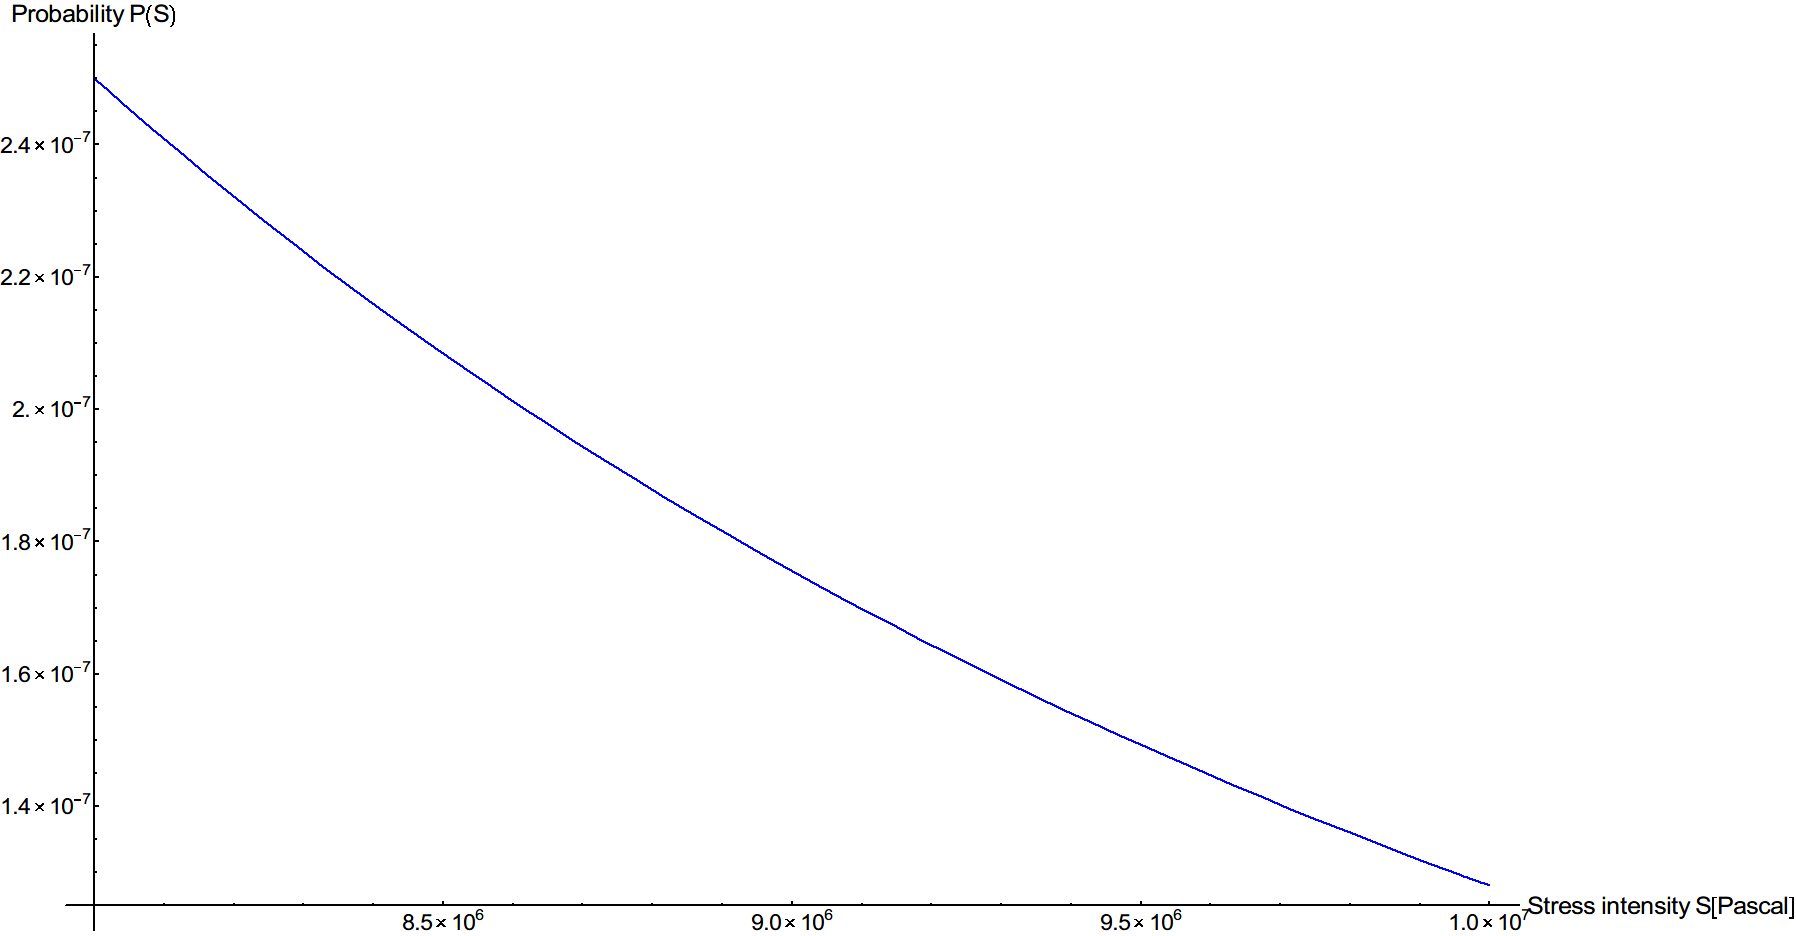
\includegraphics[width=\textwidth]{figures//distribution.png} 
		\caption{Critical distribution curve}
		\label{distribution}
\end{figure}

We assume the dissipated energy under the concentrated stress is of in the form of:

$$W_a=\frac{S^2}{k} \, for \, S>\sigma_y$$
$$W_a=0 \, for \, S<\sigma_y$$

The total dissipated energy in terms of $S$ is:
\begin{equation}
W=\int_{\sigma_y}^{\infty}P(S)W_adS=\int_{\sigma_y}^{\infty}(\beta-1)S_{max}^{\beta-1}S^{-\beta}\frac{S^2}{k}dS=\frac{(\beta-1)}{(\beta-3)}S_{max}^{\beta-1}\frac{\sigma_y^{3-\beta}}{k}
\end{equation}

If $W_F$ is the fatigue limit in the material, in stable cyclic loading we can get the number of cycles to failure as:
\begin{equation}
N_F=\frac{W_F}{W_a}=W_F\frac{\beta-3}{\beta-1}(S_{max})^{1-\beta}k\sigma_y^{\beta-3}
\end{equation}


\clearpage   

\section{Application to PSA signals}

We have a 52 minutes recording of an average customer which have driven 18.3 kilometers. A complete set of forces were recorded at the center of the left front wheel (LFW in English but RAVG in French for Roue AVant Gauche). This wheel is driving and sustains the engine mass (half of it).\\\\
FX: Force in the axial direction (from rear to front), a positive (resp. negative) force corresponds to an acceleration (resp. deceleration) of the vehicle.\\
FY: Force in the horizontal direction (from driver to shotgun), a positive (resp. negative) force corresponds to an right (resp. left) turn.\\
FZ: Force in the vertical direction (from top to bottom), a more (resp. less) than average force corresponds to a bump (resp. pot hole) in the road, the average is the vehicle mass to the wheel.\\

The summary of the signals are :

\begin{table}[h]
	\centering
	\begin{tabular}{|
			>{\columncolor[HTML]{FFFFFF}}l |
			>{\columncolor[HTML]{FFFFFF}}l |
			>{\columncolor[HTML]{FFFFFF}}l |
			>{\columncolor[HTML]{FFFFFF}}l |l}
		\cline{1-4}
\cellcolor[HTML]{34CDF9}(N) & \cellcolor[HTML]{34CDF9}max & \cellcolor[HTML]{34CDF9}mean & \cellcolor[HTML]{34CDF9}min &  \\ \cline{1-4}
		FX\_RAVG & 4739 & 113 & -3145 &  \\ \cline{1-4}
		FY\_RAVG & 2050 & 0 & -1558 &  \\ \cline{1-4}
		FZ\_RAVG & 7301 & 4012 & 1219 &  \\ \cline{1-4}
		FZ\_RARG &	5858&	3272&	647\\ \cline{1-4}
	\end{tabular}
	\caption{Summary of the signals in the center of LFW}
	\label{data}
\end{table}

\begin{figure}[h!]
	\centering
	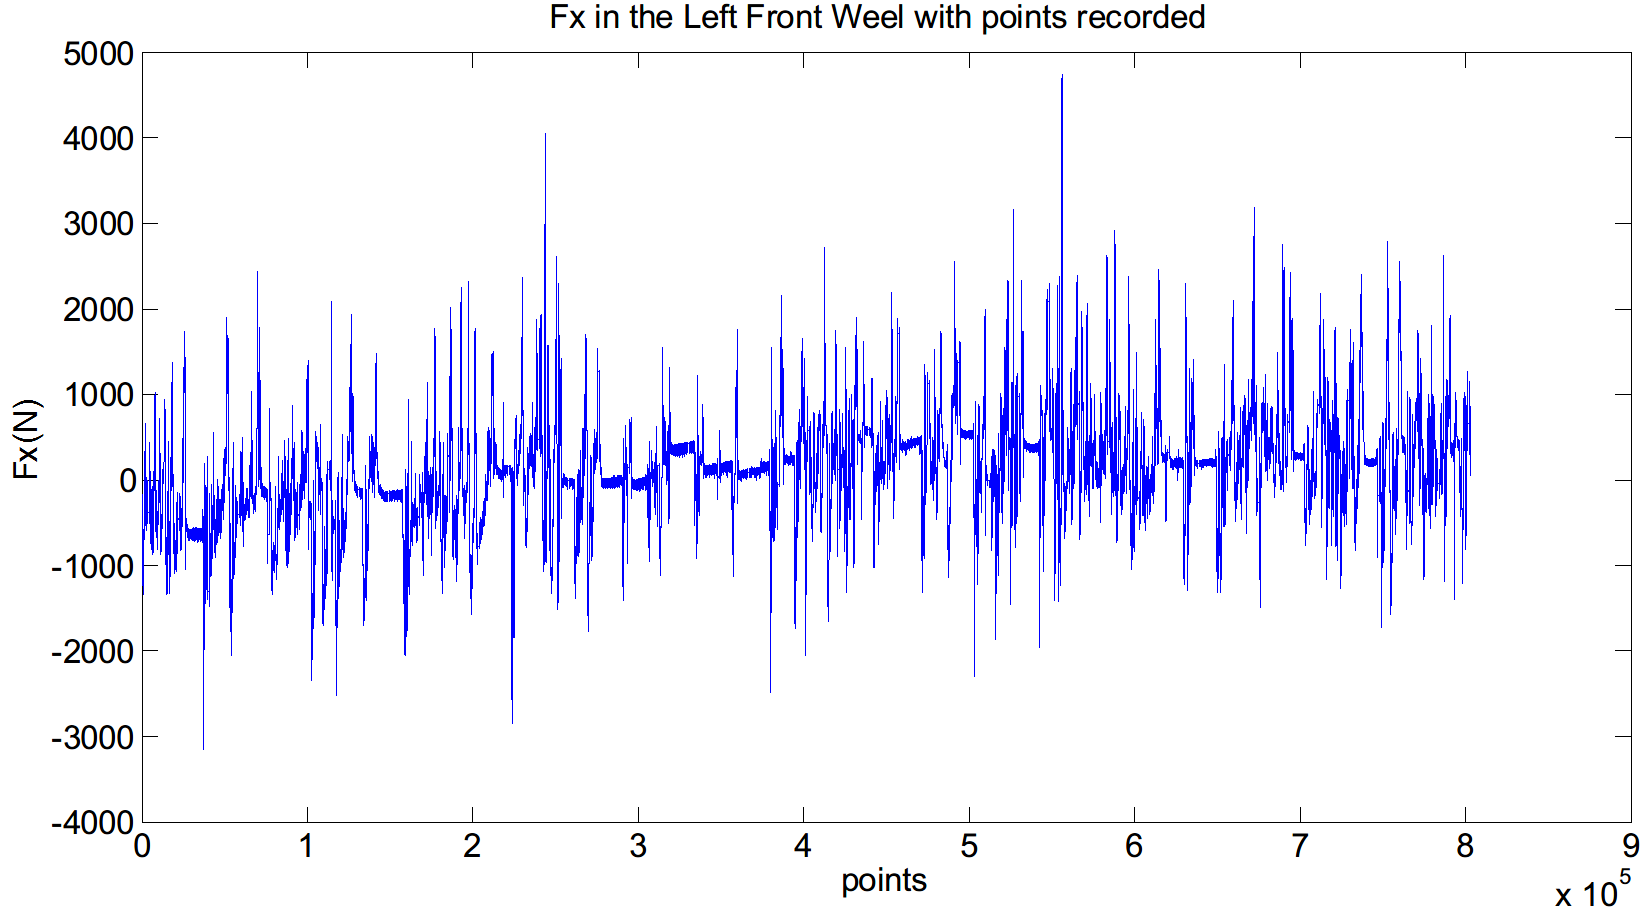
\includegraphics[width=\textwidth]{figures//fx.png} 
	\caption{Fx in the Left Front Weel with points recorded}
	\label{fx}
\end{figure}

From a comparison point of view, the rainflow counting in the Range/Mean diagram of these signals give:

\begin{table}[h]
	\centering
	\begin{tabular}{|
			>{\columncolor[HTML]{FFFFFF}}l |
			>{\columncolor[HTML]{FFFFFF}}l |
			>{\columncolor[HTML]{FFFFFF}}l |
			>{\columncolor[HTML]{FFFFFF}}l |l|}
		\hline
		\cellcolor[HTML]{34CDF9}Signal & \cellcolor[HTML]{34CDF9}nb of cycles & \cellcolor[HTML]{34CDF9}Max of Range & \cellcolor[HTML]{34CDF9}Min of Mean & \cellcolor[HTML]{34CDF9}Max of Mean \\ \hline
		FX\_RAVG & 206636 & 7884 & -3106 & 4704 \\ \hline
		FY\_RAVG & 205359 & 3608 & -1489 & 2032 \\ \hline
		FZ\_RAVG & 237703 & 6082 & 2225 & 6224 \\ \hline
		FZ\_RARG&	340967&	5211&	1482&	5122\\ \hline
	\end{tabular}
	\caption{Rainflow counting results of the force data}
	\label{rf}
\end{table}

So all the signals present a significant amounts of fatigue cycles (above 2e5) but the rear wheel is richer (by 50\%), hence it is presented here.

\section{Discussion}


\section{Conclusion}

\clearpage
\bibliographystyle{unsrt}
\bibliography{11}
\addcontentsline{toc}{section}{Reference}
\end{document}

%%
%% End of file `procs-template.tex'.
